\subsection{SUBSPACES AND PRODUCTS OF HAUSDORFF SPACES}

A subspace A of a Hausdorff space X is Hausdorff, as we see by applying Proposition 5 of no. 1 to the canonical injection A → X. Conversely, we have

PROPOSITION 6. If every point of a topological space X has a closed neighbourhood which is a Hausdorff subspace of X, then X is Hausdorff.

Let \(x \in X\) and let \(V\) be a closed neighbourhood of \(x\) in \(X\) such that the subspace \(V\) is Hausdorff. Then the closed neighbourhoods of \(x\) in \(V\) have \(\{x\}\) as their intersection (axiom \((H^i)\) ); but they are also closed neighbourhoods of \(x\) in \(X\) ( \(\S 3, no. 1\) ) and therefore \(X\) satisfies \((H^i)\) .

\pandocbounded{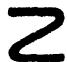
\includegraphics[keepaspectratio]{images/part001_a9a6e172.jpg}}

There exist non-Hausdorff spaces in which every point has a Hausdorff neighbourhood (Exercise 7).

PROPOSITION 7. Every product of Hausdorff spaces is Hausdorff. Conversely, if a product of non-empty spaces is Hausdorff, then each factor is a Hausdorff space.

Let \(X = \prod_{i \in I} X_i\) be a product of topological spaces. Then if \(x, y\) are two distinct points of \(X\) , we have \(\text{pr}_i x \neq \text{pr}_i y\) for some index \(i\) , and Proposition 5 of no. 1 shows that \(X\) is Hausdorff if the \(X_i\) are. Conversely, if \(X\) is Hausdorff and the \(X_i\) are non-empty, then each \(X_i\) is homeomorphic to a subspace of \(X\) ( \(\S 4\) , no. 2, Proposition 4) and is therefore Hausdorff.

COROLLARY I. Let X be a set, let \((\mathbf{Y}_{\iota})_{\iota \in \mathbf{I}}\) be a family of Hausdorff topological spaces, and for each \(\iota \in I\) let \(f_{\iota}\) be a mapping of X into \(Y_{\iota}\) . Let X carry the coarsest topology \(\mathfrak{T}\) for which the \(f_{\iota}\) are continuous. Then a necessary and sufficient condition for X to be Hausdorff is that for each pair of distinct points x, y of X we have \(f_{\iota}(x) \neq f_{\iota}(y)\) for some index \(\iota \in I\) .

The condition is sufficient by reason of Proposition 5 of no. 1. Conversely, suppose X is Hausdorff; let \(Y = \prod_{\iota \in I} Y_{\iota}\) and let \(f = (f_{\iota})_{\iota \in I}\) be the mapping \(x \to (f_{\iota}(x))\) . By Proposition 7 above Y is Hausdorff, and by Proposition 3 of §4, no. 1, \(\mathfrak{T}\) is the inverse image under f of the topology of Y. If \(f(x) = f(y)\) for two distinct points x, y of X it is clear that every open set (in the topology \(\mathfrak{T}\)) which contains x also contains y, contrary to the hypothesis that X is Hausdorff.

COROLLARY 2. Let \((\mathbf{X}_{\alpha}, f_{\alpha \beta})\) be an inverse system of topological spaces. If the \(\mathbf{X}_{\alpha}\) are Hausdorff, then \(\mathbf{X} = \varprojlim \mathbf{X}_{\alpha}\) is Hausdorff and is a closed subspace of \(\prod_{\alpha} \mathbf{X}_{\alpha}\) .

The first assertion follows from the fact that X is a subspace of the Hausdorff space \(\prod_{\alpha} X_{\alpha}\) (Proposition 7). To show that X is closed in the product space, let \(F_{\alpha\beta} (\alpha \leqslant \beta)\) be the subset of \(\prod_{\alpha} X_{\alpha}\) consisting of points x for which \(\operatorname{pr}_{\alpha}x = f_{\alpha\beta}(\operatorname{pr}_{\beta}x)\) ; the \(F_{\alpha\beta}\) are closed in \(\prod_{\alpha} X_{\alpha}\) (no. 1, Proposition 2), hence so is their intersection X.

Evidently, any sum of Hausdorff spaces (§ 2, no. 4, Example 3) is a Hausdorff space.

